\documentclass{article}
\usepackage[en]{ukon-infie}
\usepackage[utf8]{inputenc}
\usepackage{algorithm2e}
\usepackage{amsmath}
\usepackage{graphicx}
% kann de oder en sein
% kann bubble break, topexercise sein

\Names{Jonas Probst, Simon Giebenhain, Gabriel Scheibler, Clemens Gutknecht}
\Lecture[DLCV]{Deep Learning for Computer Vision}
\Term{WS 2017/18}

\begin{document}
    \begin{ukon-infie}[3.12.17]{2}

		
		\begin{exercise}[p=45]{}
			\question{}{
			We normalized in two different ways:\\
			\textbf{zero mean and unit norm:}\\
			Subtract the mean of an image from every pixel of that image, such that the image has zero mean. Then divide each pixel by the L2-Norm of the image. With this method we the fully trained logistic regression achieved roughly 78\% accuracy.\\
			
			\textbf{zero mean and sigmoid:}\\
			The first step is the same. But then a slightly modified sigmoid function is applied to every pixel, in order to increase the contrast in the picture and reduce some noise. With this method we the fully trained logistic regression achieved roughly 80\% accuracy. The following picture shows the result of this normalization for the first 5 images.\\
			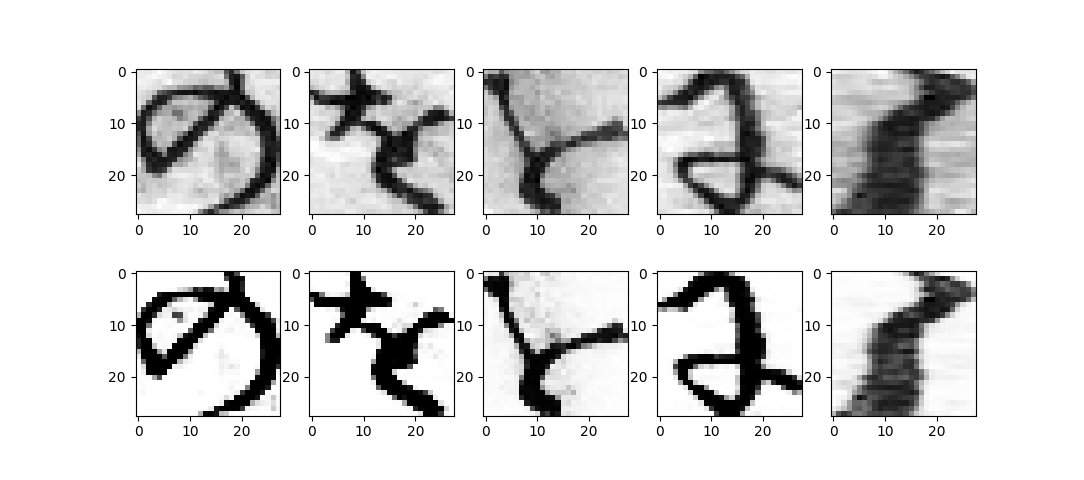
\includegraphics[scale=0.6]{sigmoid_normalization.png}\\
			
			}
			\question{}
			{
			For details see \textbf{logistic\_regression.py}.	
			The best test accuracy we achieved was just above 80\%}
			\question{}
			{
			In the follwong picture one column represents one class. The uppermost row is an illustration of the weights, which were trained in the logistic regression above (sigmoid normalization). The other images are just examples from this class.\\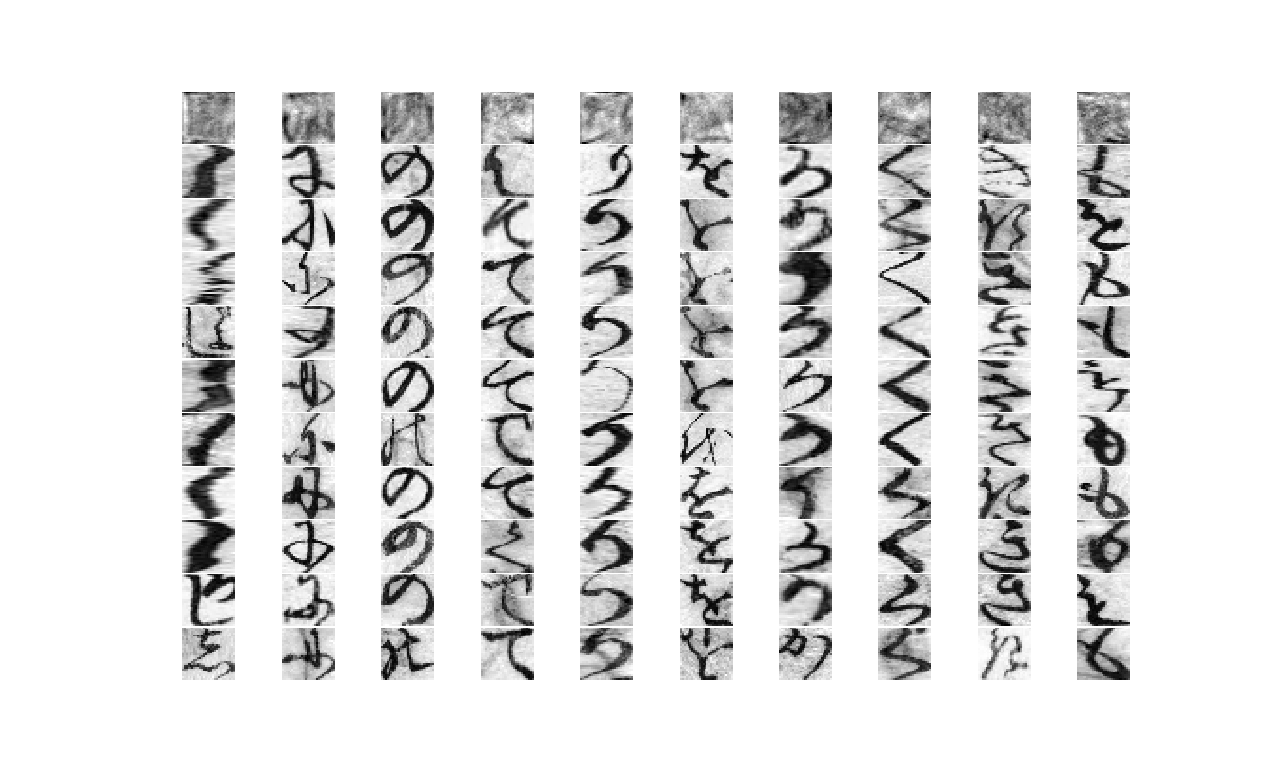
\includegraphics[scale=0.5]{weights.png}}   \\	
			Altough the weights may seem somewhat random at first glance, one observes (strong) structral similarities between the weights and the pictures of the class. The most obvious are  illustrated below:\\
			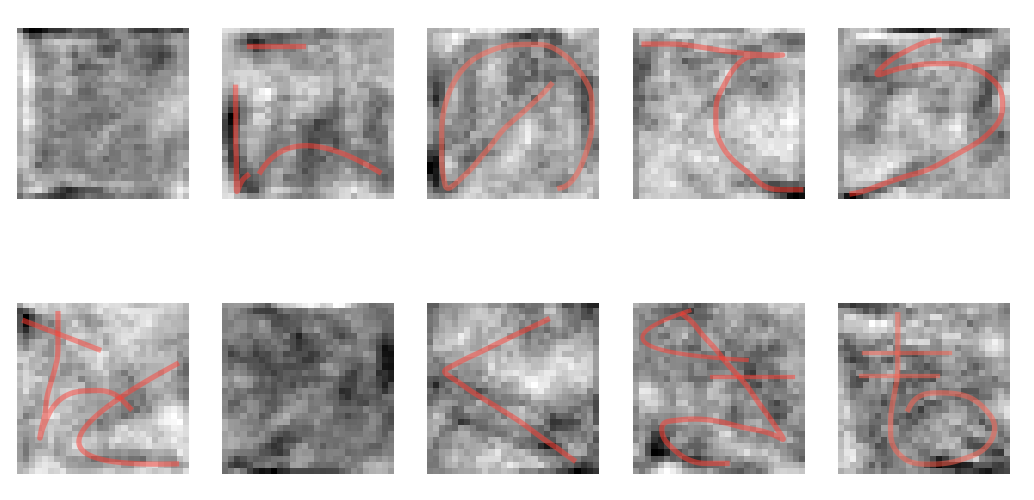
\includegraphics[scale=0.5]{weights_similarities.png}
		\end{exercise}
		
		\begin{exercise}[p=55]{}
			\question{}{
			We besed our network design on the google tutorial.\\
			The source code of this and all of the following subexercises can be found in \textbf{deep.py}}
			\question{}
			{
			We used the sigmoid normalization as desribed above, instead of the unit norm, because this yielded slightly better results.\\
			Our batches for the training contained 43 images each. The corresponding method is \textbf{run\_standar\_version()}.
			}
			\question{}{
			train accuracy: 99.995\%\\
			test accuracy: 97.496\%}
			\question{}{
			When we removed the second convolutional layer, we obtained the following results:\\
			train accuracy: 99.970\%\\
			test accuracy: 96.101\%\\
			
			We see that while the train accuracy hardly changes, the test accuracy deteriorates more severely. Therefore we conclude, that removing one layer causes the model to  lose some ability to generalize. This can be explained by the more shallow structure of the convolutional network. It does not combine the features of layer 1 to bigger features (because that layer has been lost). Therfore the model has a worse internal representation and smaller receptive field.
			}
			\question{}{
			We chose to use the more sophisticated AdamOptimizer instead of the GradientDescentOptimizer, like it was recommended in the Google tutorial. \\
			The following graph, shows the development of the test accuracy with training cycles ranging from 0 to 15.000 for different step sized, which varied from 1 to $10^{-6}$.\\
			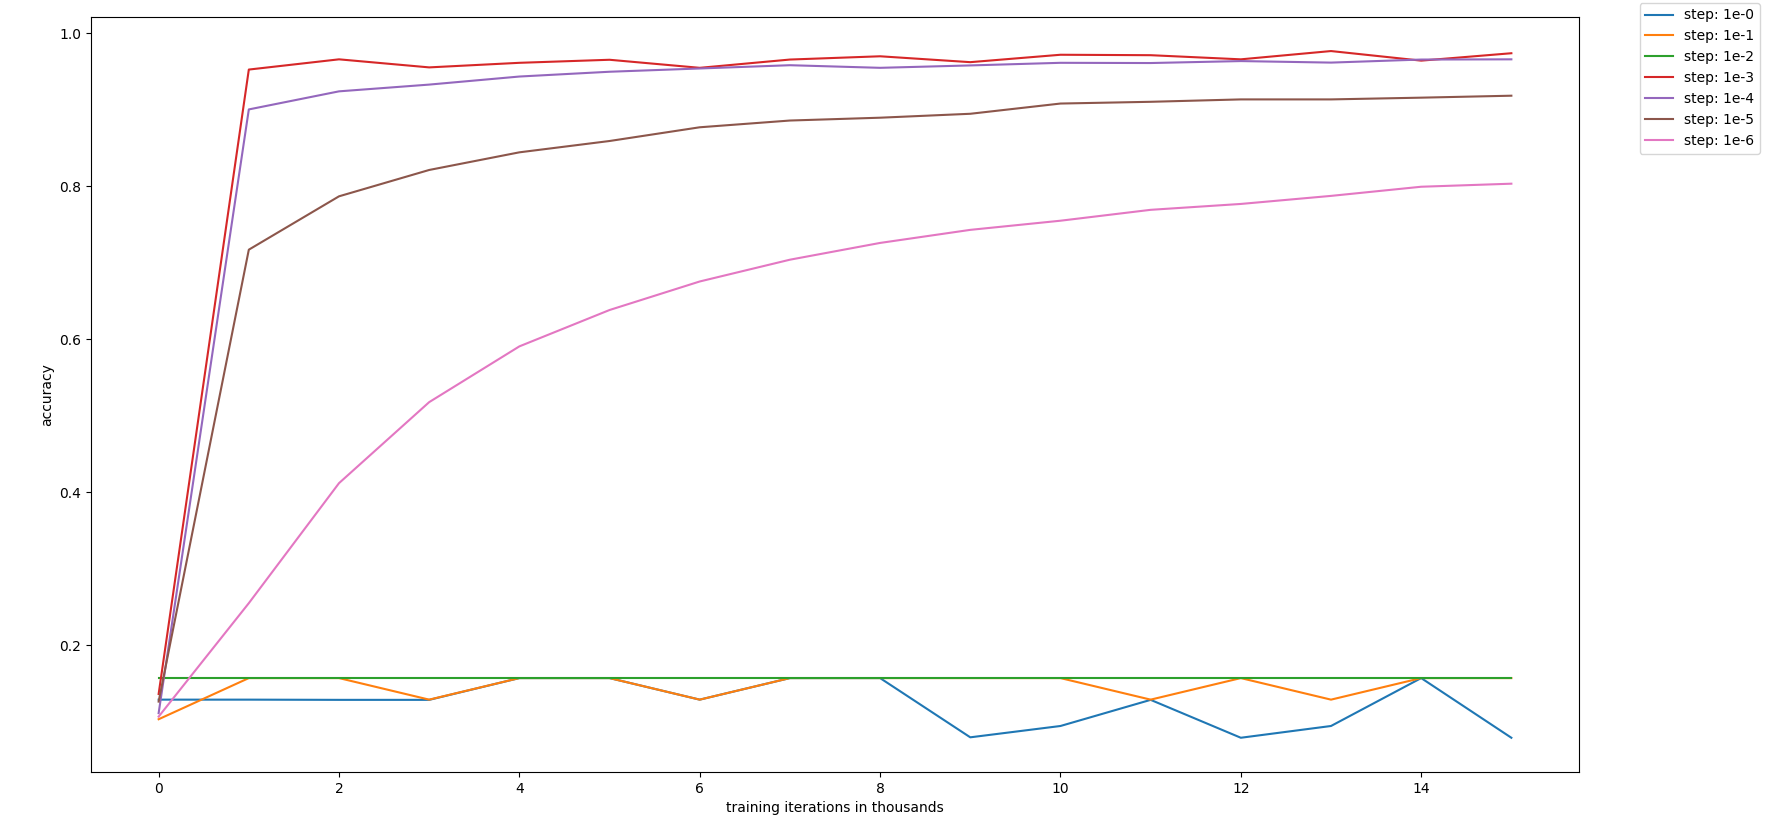
\includegraphics[scale=1.2]{step.png}\\
			
			One observes that the bigger step sizes (1, 0.1 and 0.01) are way to coarse, such that the optimizer jumps back and forth over local minima.\\
			Decreasing the step size just a little bit (to $10^{-3}$ or $10^{-4}$), makes huge improvments in accuracy. These step sizes seem to fit the problem quite well. With the first 1000 training cycles their accuracy rises extremely fast. It almost seems that for step size $10^{-3}$ a local minima has already been found, as the accuracy only improves slightly and does this in a zig-zag fashion. For step size $10^{-4}$ it takes up to 6000 training cycles to reach a local minima. However the accuracy curve is much smoother as for $10^{-3}$, because of the slightly smaller step size.\\
			
			Further decreasing of the step size, causes to model to learn more slowly. Furthermore the models cannot jump accross local minima as good as before, which causes them to get stuck in worse local minima than before. The corresponding function in \textbf{deep.py} is \textbf{step\_size()}.
			
			}
			\question{}{
			We played around with some of the hyper-parameters for quite some time. We did 4-fold cross validation. However for a lack of computational power, we decided to only evalute their influence one at a time (instead of checking all combinations of hyper-parameters.) This means that for each hyper-parameter we kept all other hyper-parameters the same as in the exercises before. This means that our evaluation of the hyper-parameters is only in the context of the base parameters. These base hyper-parameters are the following:\\
			
\begin{tabular}{|l|l|l|l|l|l|}
\hline
kernel size                 & \#features  1 & \#features2 & pooling                 & dropout & \#fully connected \\ \hline
5x5, zero padding, stride=1 & 32            & 64          & max\_pool 2x2, stride 2 & 0.5     & 1024              \\ \hline
\end{tabular} \\
			
			\textbf{Size of the fully layer}:\\
			Here the training and testing accuracy for changing sizes of the fully connected layer are displayed. \\
			It can be seen that with small fully connected layers, there is underfitting to a certain degree and with too many nodes there is some overfitting. There seems to be a local maximum somewhere between 512 and 2048. However we did not have enough time for further investigations.\\
			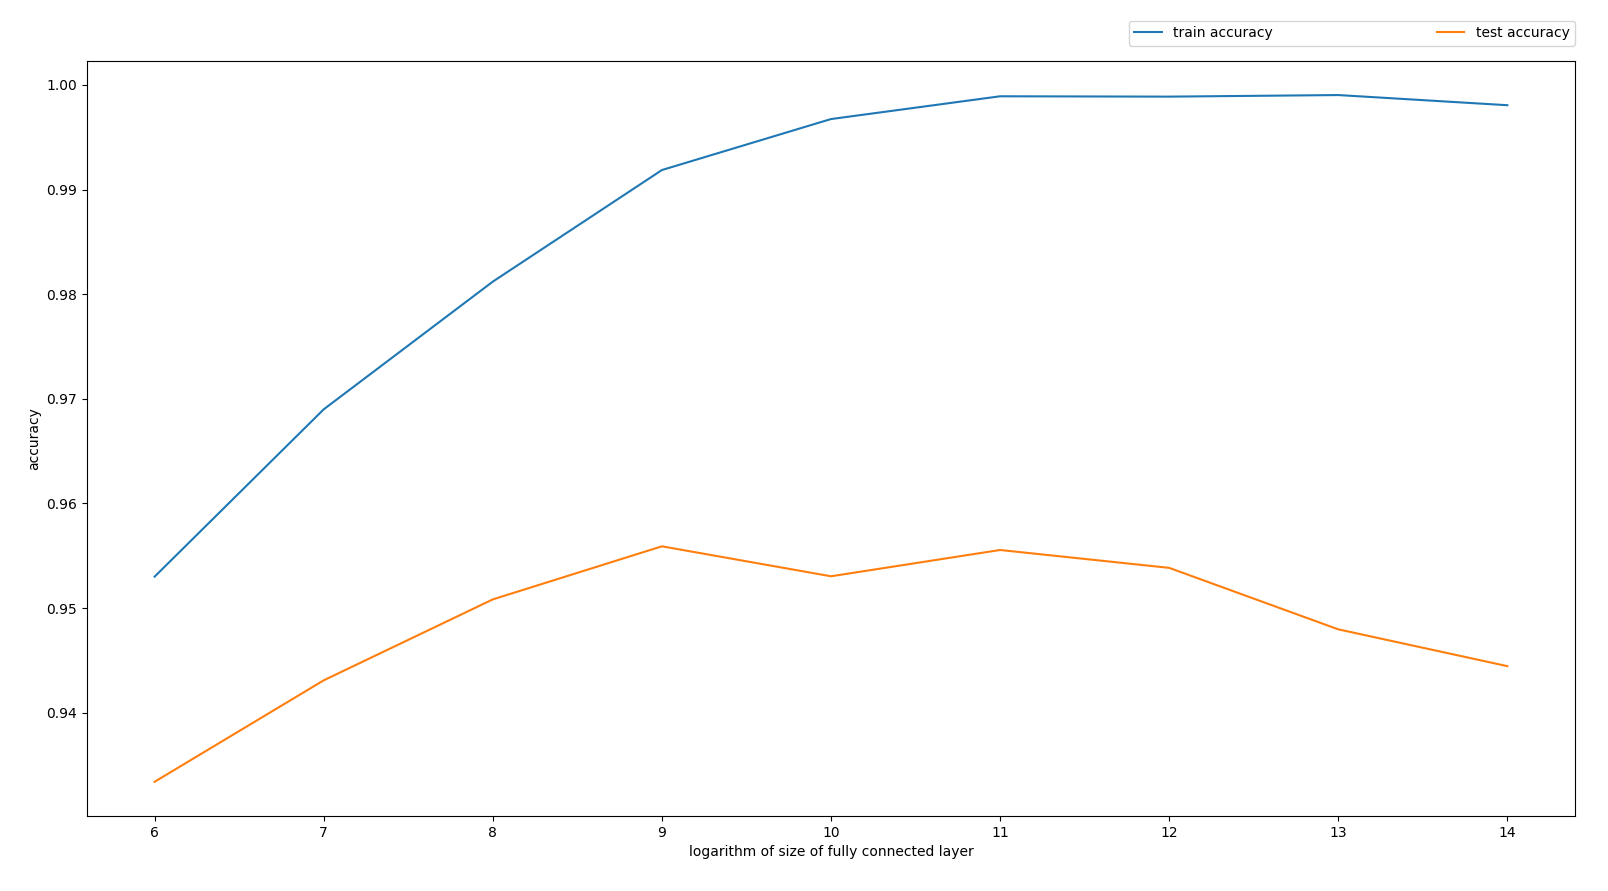
\includegraphics[scale=1.1]{convsize.png}\\
			
			
			\textbf{Size of kernels:} 
			We compared 3x3, 5x5, and 7x7 kernels and it seems that 7x7 is too big for our images and 5x5 might be slightly worse than 3x3.\\
			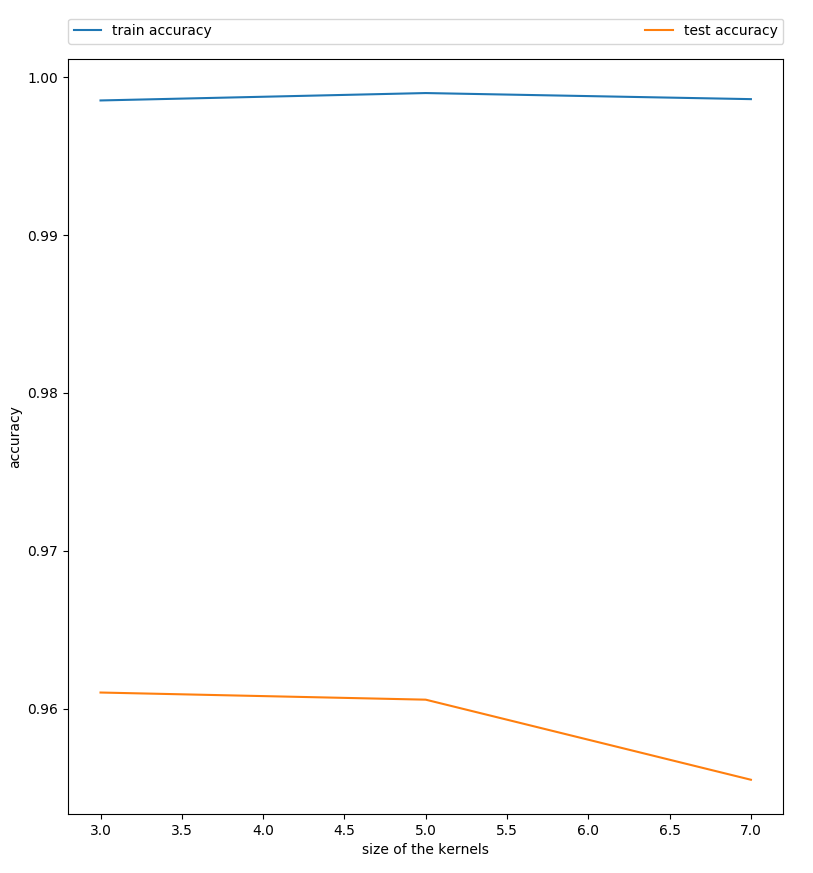
\includegraphics[scale=1.1]{kernelsize.png}\\
			

			\textbf{Number of features in the convolutional layer:}\\
			
			We compared different numbers of features for the first convolutional layer ranging from 4 to 128. The second convolutional layer had double the number of features of the first layer. The results show that a local optimum lies somwhere around 32. With below 32 features the model's capacity was to low for a high accuracy. With more features than 32 the test accuracy decreased again. However the training accuracy decreased equally. This might indicate that the number of training cycles(12500) was not sufficient to fully train that much features.\\
			
			\includegraphics[scale=0.6]{hyper_nr_features.png}\\
			
			\textbf{Number of 3x3 convolutions replacing single convolution:}
			Here we stacked some multiple 3x3 convolutional layers in order to replace the 5x5 convolution.\\
			Our testing considered the following configuration (1:1), (1:2), (2:2), (2:3) and (3:3), where the first digit represents the size of the stack replacing the first convolutional layer and the second digit the second one. (2:3) achieved the best test result, altough it wasn't fully trained yet. It seems that with increasing stack sizes the networks take longer to train. (Training was done with 12500 cycles.)\\
			
			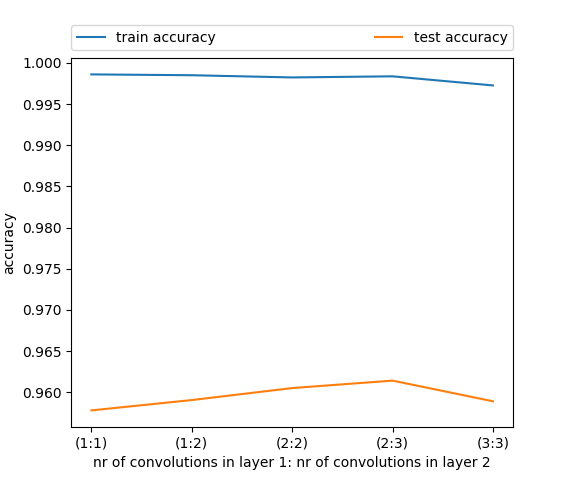
\includegraphics[scale=0.5]{hyper_nr_convolutions.png}
			\\
			The remaing methods in \textbf{deep.py} are dedicated towards this exercise. 
			}
		\end{exercise}
		\begin{exercise}[p=20]{}
		\question{}{
			We saved the weights of our fully trained model in \textbf{save\_weights.py}.\\
			In \textbf{retrain\_on\_mnist.py} we restore all these weights in nontrainable variables except for the variables in the fully connected layer. These remain trainable.\\
			For the details of the implementation see  \textbf{save\_weights.py} and \textbf{retrain\_on\_mnist.py}.
		}
		\question{}{
			
We retrained in two different fashions. Once we retrained only the outgoing weights of the fully connected layer and once we retrained the complete fully connected layer. We obtained the following results:\\

Accuracy when retraining in- and output-weights of the fully connected layer: 99.10\% \\
Accuracy when only retraining output-weights of the fully connected layer: 97.86\% \\

In comparison here are the results when training completley on MNIST:\\

Accuracy for the logistc regression model fully trained on MINIST: 92\% \\
Accuracy for the convolutional model fully trained on MINIST: 99.7\% \\
			
Comparing the results of the retrained network with the convnet, which was completely trained on MNIST one observes the follwoing:\\
Altough the features were trained on the japanese characters, they could also be used to relatively accurately classify MINIST data(0.6\% loss in accuracy in comparison to the convnet on MNIST), even though much less parameters had to be trained. Therefore one concludes, that the feature extraction trained on the japanese characters largly transfers for classifying arabic digits.\\

Comparison of the retrained network vs. logistic regression:\\
Considering that the amount of weights you have to train when only retraining output-weights of the fully connected layer($1024 \cdot 10$) is only slightly bigger than the amount of weights in the regression model($728 \cdot 10$), it seems way more efficient to retrain the fully connected layer, looking at the difference in achieved accuracy of these two options.\\		}
		\end{exercise}
		\begin{exercise}[p=20]{}
		
		The following picture shows the unit response for all classes. The images were obtained as an an average over 25 single results, each computed as described on the exercise sheet.\\
		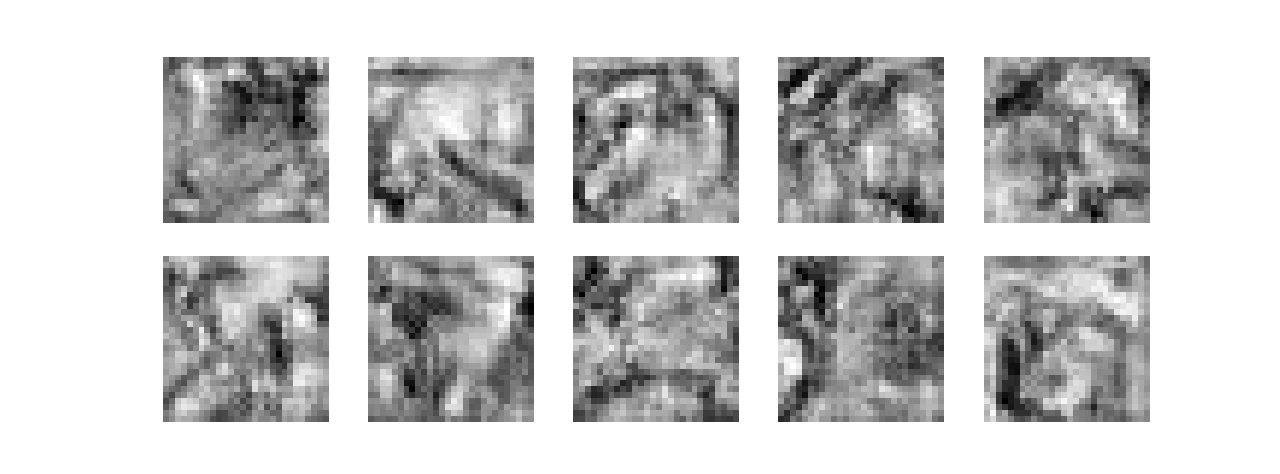
\includegraphics[scale=0.5]{unit_resonse_final_layer_avg25.png}
		
		The following picture depicts the unit respnse of the first convolutional layer. However the settings with which it was computed did not work for every feature at the same time (for some the value deverged to negativ infinty). Nevertheless a good amount resembles Gabor filters.
		
		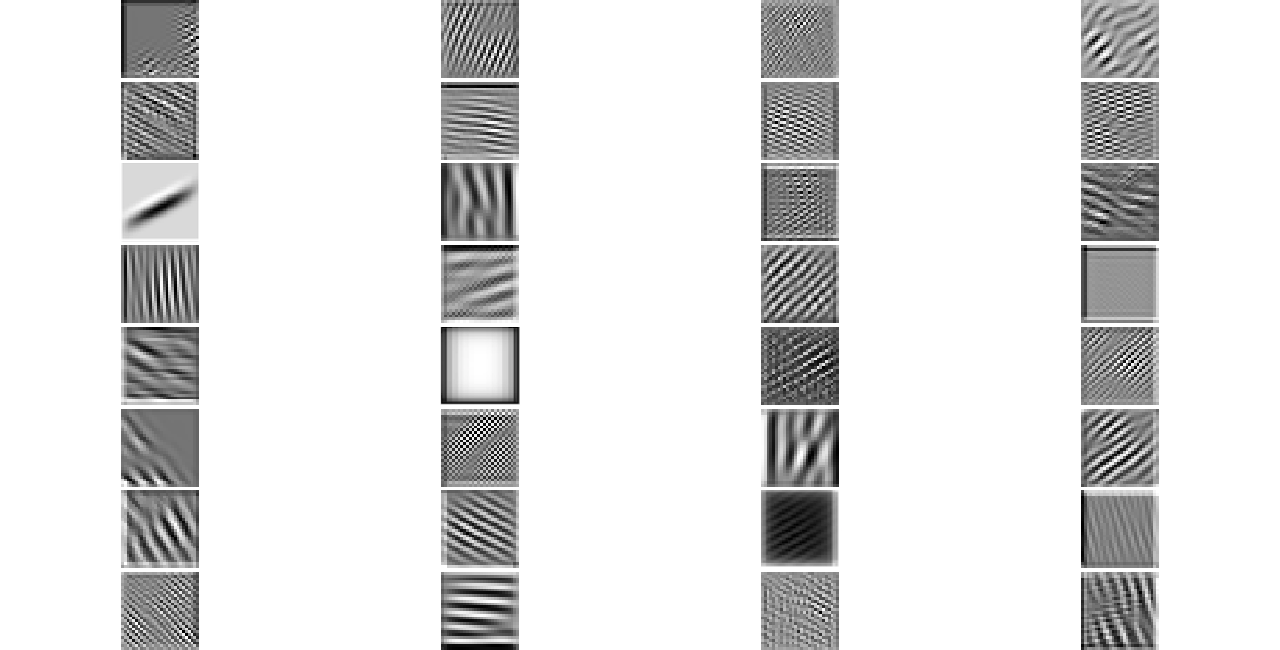
\includegraphics[scale=0.5]{resp_conv1.png}
		
		The source can be found in \textbf{response.py}.
				
		\end{exercise}
		\begin{exercise}[p=20]{}
		Since the random samples are uniformly drawn, it is clear that they can only be natural numbers (not real valued).\\
		
		\question{}
		{
				In order to check the bias of the estimator $\overline{x}$, we need to compute the expected value for $\overline{x}$ over all possible samples:\\

		\begin{eqnarray*}
		bias(\overline{x}) 
		&=& E_{x_1, \dots, x_L \in [0, \theta]}[\overline{x}] - \theta \\
		&=& E_{x_1, \dots, x_L \in [0, \theta]}\left[\frac{1}{L}\sum_{l = 1}^L x_l\right] - \theta \\
		&\stackrel{E ~ linear}{=}& \frac{1}{L}\sum_{l = 1}^L E_{x_l \in [0, \theta]}[x_l] - \theta \\
		&=& \frac{1}{L}\sum_{l = 1}^L \frac{1}{\theta + 1}\sum_{i = 0}^{\theta} i - \theta \\
		&=& \frac{1}{L}\sum_{l = 1}^L \frac{\theta \cdot (\theta + 1)}{2 \cdot (\theta + 1)} - \theta \\
		&=& \frac{1}{L}\sum_{l = 1}^L \frac{\theta }{2} - \theta \\
		&=& \frac{\theta }{2} - \theta \\
		&=& \frac{-\theta }{2}\\
		&\not =& 0 \\
		\end{eqnarray*}
		
		Therefore $\overline{x}$ is biased (unless $\theta = 0$).
		}
		
		\question{}
		{
			Let $\hat{\theta}(x) := 2\overline{x}$. Then the following holds:\\
			$bias(\hat{\theta}(x)) = bias(2 \overline{x}) = E[2 \overline{x}] - \theta \stackrel{E ~linear}{=}2 E[\overline{x}] - \theta = 0$
		}
		
		\question{}
		{
			\begin{eqnarray*}
			var(\hat{\theta}(x))
			&=& E\left[(\hat{\theta}(x) - E[\hat{\theta}(x)])^2\right] \\
			&=& E\left[\left(\frac{1}{L}\sum_{l = 1}^L 2x_l - \theta\right)^2\right] \\
			&=& E\left[\frac{1}{L^2}\sum_{l = 1}^L\sum_{k=1}^L (2x_l - \theta)(2x_k - \theta)\right] \\
			&=& \frac{1}{L^2}\sum_{l = 1}^L\sum_{k=1}^L E\left[(2x_l - \theta)(2x_k - \theta)\right] \\
			&\stackrel{*}{=}& \frac{1}{L^2} \sum_{l = 1}^L E\left[(2x_l - \theta)^2\right] \\
			&=& \frac{1}{L^2} \sum_{l = 1}^L var(2x_l) \\
			&\stackrel{**}{=}&\frac{1}{L^2} \sum_{l = 1}^L \sigma^2 \\
			&=& \frac{L \sigma^2}{L^2}  \\
			&=& \frac{\sigma^2}{L}  \\
			\end{eqnarray*}
			Therefor it follows that $stderr(\hat{\theta}(x)) = \frac{\sigma}{\sqrt[2]{L}}$.\\
			And since $\sigma$ is independent of the sample size and $\lim_{L \to \infty} \sqrt[2]{L} = \infty$ it follows:\\
			$\lim_{L \to \infty} stderr(\hat{\theta}(x)) = 0$
			
			In the proof above there are still 2 points to discuss:\\
			
			\textbf{**}: $var(2x_l) = E_{x_l \in [0,\theta]} (2x_l - \theta)^2$. The sample size is not involved, so the $\sigma$ is independet of $L$. Furthermore the variance is the same for all $x_1, \dots x_L$.\\
			
			\textbf{*}: The duoble sum in this equation $\frac{1}{L^2}\sum_{l = 1}^L\sum_{k=1}^L E\left[(2x_l - \theta)(2x_k - \theta)\right] $, iterates over all covariances. Since $x_1, \dots x_L$ are drawn independently from $[0, \theta]$, the covaraince is 0, except $k=l$.
			
		}
		
		\question{}
		{
			Let $\hat{\theta}(x) := max(x)$. First let's show that $\hat{\theta}$ is biased with induction:\\
			\textbf{Induction Base:}\\
			Let $L=1$. $E_{x \in [0,\theta]}[\hat{\theta}] = E[max(x)] = \frac{1}{\theta + 1} \sum_{i = 0}^{\theta}i = \frac{\theta}{2}$.\\
			
			\textbf{Induction Step:}\\
			Let $L\in \mathbb{N}^+$. \\
			$E_{x_1 \in [0,/theta], \dots x_{L+1} \in [0,\theta]}[max\{x_1, \dots, x_{L+1}\}] = E[max\{max\{x_1, \dots x_L\}, x_{L+1}\}] \stackrel{ind. hyp.}{=}E[max\{\frac{\theta}{2}, x_{L+1}\}] = max\{\frac{\theta}{2}, E_{x_{L+1}\in [0,\theta]}[x_{L+1}]\} = max\{\frac{\theta}{2}, \frac{\theta}{2}\} = \frac{\theta}{2}$. \\
			It follows that $bias(\hat{\theta}) = \frac{-\theta}{2}$. Thus $\hat{\theta}$ is bias unless $\theta = 0$.
			
			Now let's figure out the standar error:\\
			
			
			\begin{eqnarray*}
			var(\hat{\theta}(x)) 
			&=& E[(max(x) - E[max(x)])^2] \\
			&=& \sum_{i = 0}^{\theta} P(max(x) = i) (i - E[max(x)])^2 \\
			&=& \sum_{i = 0}^{\theta} P(max(x) = i) (i - \sum_{j = 0}^{\theta}P(max(x) = j) j)^2
			\end{eqnarray*}
			\\
			 Now consider $L \rightarrow \infty$: \\
			$\lim_{L \to \infty} P(max(x) = i) = \lim_{L \to \infty} P(max\{x_1, \dots x_L\} = i)  ~ = \begin{cases}
     1 & \text{if} ~ i = \theta \\
     0 & \text{else} 
   \end{cases}$.
   Therefore the equation above reduces to teh following:\\
   $\sum_{i = 0}^{\theta} P(max(x) = i) (i - \sum_{j = 0}^{\theta}P(max(x) = j) j)^2 = (\theta - \theta)^2  = 0$
   \\
   Since the $\lim_{L \to \infty}var(\hat{\theta}) = 0$, the same holds for the standdard error.
		}
		\end{exercise}
		
		
\end{ukon-infie}
\end{document}
